%==========================================================================================
\section{Related Work}

\subsection{The Canonical SLAM Problem}
Given an accurate map of an environment, it is relatively straightforward to localize based on the features. Conversely, given accurate localization (for instance, by perfect dead reckoning), it is relatively straightforward to construct a map. However, taking neither as given turns this into a ``chicken and egg'' problem, called simultaneous localization and mapping (SLAM). In order to resolve this, we define a state vector of both the vehicle configuration and the observed landmarks thus far: \cite{corke}

\begin{equation*}
    \hat{\mathbf{x}} = (x_v,y_v,\theta_v,x_1,y_1,x_2,y_2, \ldots x_M, y_M)^T \in \mathbf{R}^{(2M+3) \times 1 }
\end{equation*}

The covariance estimate of this vector is:

\begin{equation*}
    \hat{\mathbf{P}} = \begin{bmatrix}
        \hat{\mathbf{P}}_{vv} & \hat{\mathbf{P}}_{vm} \\
        \hat{\mathbf{P}}_{vm}^T & \hat{\mathbf{P}}_{mm}
    \end{bmatrix}
\end{equation*}

wherein $\hat{\mathbf{P}}_{vv}$, $ \hat{\mathbf{P}}_{mm}$, and $\hat{\mathbf{P}}_{vm}$ are the covariances of the vehicle pose, landmark positions, and correlation between pose and landmarks, respectively. An extended Kalman filter can be used to predict and update the state and covariance.

New landmarks can be incorporated by extending the covariance matrix:
\begin{equation*}
    \hat{\mathbf{P}}\langle k \rangle ' = \mathbf{Y_z}\begin{bmatrix}
        \hat{\mathbf{P}} \langle k \rangle & 0\\
        0 & \hat{\mathbf{W}}
    \end{bmatrix} \mathbf{Y_z}^T
\end{equation*}

wherein $\hat{\mathbf{W}}$ is an estimate of the sensor covariance and $\mathbf{Y_z}$ is the so-called ``Insertion Jacobian", given by: \begin{equation*}
    \mathbf{Y_z} \equiv \frac{\partial \mathbf{y}}{\partial \mathbf{z}} = \begin{bmatrix}
        \mathbf{I}_{n \times n} & & \mathbf{0}_{n\times 2} \\
        \mathbf{G}_x & \mathbf{0}_{2\times n-3} & \mathbf{G}_z
    \end{bmatrix}
\end{equation*}

wherein $\mathbf{G}_z$ and $\mathbf{G}_x$ are the partial derivatives of the function $\mathbf{g}$ which gives the coordinates of an observed landmark based on known vehicle pose.

However, implementing SLAM requires a way to associate landmarks with locations in space. In the case of visual SLAM, feature recognition from a camera image is used to determine the landmarks to be used. This will be discussed further in the section below.

%------------------------------------------------
\subsection{ORB-SLAM}

\begin{figure}[H]
    \centering
    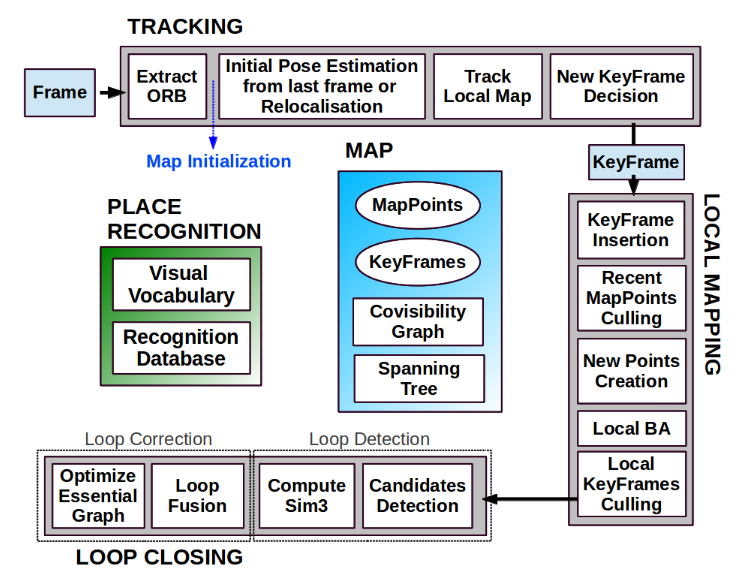
\includegraphics[width=\columnwidth]{figures/ORBSLAMoview.png}
    \caption{Overview of the ORB-SLAM system \cite{ORBSLAM}}
    \label{fig:OSLAMOview}
\end{figure}

The specific SLAM solution we implemented was the ORB-SLAM monocular visual SLAM algorithm, as proposed by Mur-Artal et. al. \cite{ORBSLAM} and summarized in Figure \ref{fig:OSLAMOview}.

In order to allow real-time performance without reliance on onboard GPUs or other co-processing units, ORB-SLAM bases its feature detection around so-called ``ORB features" as introduced by Ruble et. al. \cite{ORB} which are far less computationally expensive than SIFT or SURF detection.

The ORB-SLAM algorithm can be divided into three major sub-steps: tracking, local mapping, and loop closing, each of which is discussed in the following subsections.

%------------------------------------------------
\subsubsection{Tracking}

When a frame is input to the algorithm, first the ORB features are extracted. Next, these features are compared to the previous frame in order to estimate pose. Once this estimate is completed, the map is projected onto the new frame and we search for correspondences between the map and the frame. Finally, we decide if the current frame should be used as a keyframe going forward based on the number of points tracked, the similarity of those points to the previous keyframe, and the time since the last keyframe was spawned.

%------------------------------------------------
\subsubsection{Local Mapping}

This process is performed only if a new keyframe is added in the final step of the tracking process. First, the new keyframe is added to the covisibility graph and linked to the other keyframe which has the most points in common. Next, a bag of words representation for this keyframe is computed. After this, points in the map are tested to determine whether they are ``good enough'' to retain, or if they should be culled. This standard of ``good enough'' is determined based on two criteria. First, the algorithm predicts, from the position of the map point, in which other keyframes it should have been visible, and checks if it was visible in those frames. So long as it is found in over $25\%$ of them, it is not rejected. Second, it must also appear in at least three other keyframes, although this condition is skipped when first initalizing the map as it would otherwise prevent the inclusion of any points in the map.
Next, the ORB features from the new keyframe are triangulated with each of the connecting keyframes in the covisibility graph. For each unmatched ORB, we can simply search for matches within the set of unmatched ORBs in the other keyframes. Finally, a local bundle adjustment is performed to optimize the covisibility graph.
As an optional step, we can discard keyframes which have too many points in common with too many other keyframes. This can help to keep the model lightweight and reduce the processing required.

%------------------------------------------------
\subsubsection{Loop Closing}

With our new keyframe having been added in the previous step, we can now proceed to Loop Closing. Using the Bag of Words representation as previously calculated, we compare the similarity of the newest keyframe to each of its neighbors in the covisibility graph. The lowest of these similarities is saved. Any of the previous keyframes whose saved value is lower than that of our newest keyframe is retroactively discarded in order to improve robustness of the algorithm. Loop candidates must have three frames in a row which are mutually consistent.

We first compute ORB correspondences between the current keyframe and the loop candidates, which give 3D to 3D correspondences. We use these results to fuse the duplicated map points and insert new edges into the covisibility graph. The new keyframe is corrected with a similarity transform, and this correction is propagated to the keyframe's neighbors in the covisibility graph. Map points seen by the loop keyframe are similarly projected into the new keyframe that is being added and its neighbors. Any matches found in this projection are subsequently fused and all keyframes with fused map points have their edges updated correspondingly, thus concluding the loop closure and the ORB-SLAM algorithm.
